\chapter{Примененеие диаграмной техники}

Возвращаясь к раскладке неразличимых предметов по неразличимым ящикам. Уравнение, к решению которого сводится исходная задача:
\[
	\begin{split}
		& x_1 + x_2 + ... + x_k = n \\
		& x_1 \ge x_2 \ge ... \ge x_k > 0
	\end{split}
\]

Рассмотрим свойства известных нам чисел $p_k\left(n\right)$:
\begin{enumerate}
\item $p_1\left(n\right) = 1$

\item $p_2\left(n\right) = \lfloor n/2\rfloor$

\item $p_n\left(n\right) = n$
\end{enumerate}

Утверждаем, что 
\[
	\begin{split}
		&p_k\left(n\right) = \sum_{r=1}^{m} p_r\left(n-k\right)\\
		&m = min\{k, n-k\}
	\end{split}
\]

Рассмотим случаи. Первый случай $k\ge n-k \Leftrightarrow k/2 \ge n$:
\[
	\begin{split}
		&p_k\left(n\right) = \sum_{r=1}^{m} p_r\left(n-k\right) = \sum_{r=1}^{n-k} p_r\left(n-k\right) = p\left(n-k\right)
	\end{split}
\]
но это и так очевидно, так как $p_k\left(n\right) = p\left(n-k\right)$ (из комбинаторных соображений, пусть есть разбиение $n-k$ предметов по не более чем $k$ ящикам, разложим в каждый ящик по 1 редмету и получим разбиение $n$ предметов ровно по $k$ ящикам, и в обратную сторону). Таким образом в одном случае утверждение доказано.

Второй случай $k < n-k$. $p_k\left(n\right) = \sum_{r=1}^{k} p_r\left(n-k\right)$. Покажем это любимым методом разделения. Рассмотрим какие варианты возможны, если мы уберем из каждого из $k$ ящиков по одному предмету, то получим разложение $n-k$ предметов по не более чем $k$ ящикам, просуммируем по всем количествам непустых вариантов и полуим требуемое.

Итого утверждение доказано.

Теперь пользуясь этой странной и неудобной штукой получим прикольную и удобную штуку.

Пусть $1 \le k \le n/2 \Leftrightarrow k \le n-k$, тогда справедливо:
\[
	p_k\left(n\right) = \sum_{r=1}^{k-1} p_r\left(n-k\right) + p_k\left(n-k\right)
\]
а кроме того:
\[
	p_{k-1}\left(n-1\right) = \sum_{r=1}^{k-1} = p_r\left(n-1-k+1\right) = \sum_{r=1}^{k-1} p_r\left(n-k\right)
\]
собираем все вместе:
\[
	p_k\left(n\right) = p_{k-1}\left(n-1\right) + p_k\left(n-k\right)
\]
Теперь проверим, что и при $k>n-k$ полученное соотношение так же справедливо:
\[
	\begin{split}
		& p_k\left(n-k\right) = 0 \\
		& p_k\left(n\right) = \sum_{r=1}^{k-1} p_r\left(n-k\right) + p_k\left(n-k\right) = p_{k-1}\left(n-1\right) + p_k\left(n-k\right)
	\end{split}
\]

А это уже удобное рекуррентное соотношение, которое можно доказать и комбинаторно. Для этого нужно разбить все раксладки $n$ неразличимых предметов ровно по $k$ ящикам на блоки в которых присутствует ящик с ровно одним предметом и разбиения без таких ящиков, и получаем требуемое.

Теперь рассмотрим задачу о разложении по не более чем $k$ ящикам ($P_k\left(n\right)$). Для таких чисел справедливы следующие соотношения:
\begin{enumerate}
\item $P_n\left(n\right) = p\left(n\right)$

\item $P_1\left(n\right) = 1$

\item $\forall k \ge 1 : P_k\left(0\right) = 1$

\item $P_k\left(n\right) = p\left(n\right)$, при $k>n$

\item $P_k\left(n\right) = \sum_{r=1}^k p_r\left(n\right) \Rightarrow p_k\left(n\right) = P_k\left(n\right) - P_{k-1}\left(n\right)$
\end{enumerate}

Получим рекуррентное соотношение для этих чисел:
\[
	\begin{split}
		&P_k\left(n\right) = \sum_{r=1}^k p_r\left(n\right) = \sum_{r=1}^{k-1} p_r\left(n\right) + p_k\left(n\right) = \\
		& = P_{k-1}\left(n\right) + p_k\left(n\right) = P_{k-1}\left(n\right) + \sum_{r=1}^m p_r\left(n-k\right) = \\
		& = P_{k-1}\left(n\right) + P_m\left(n-k\right) = P_{k-1}\left(n\right) + P_k\left(n-k\right)
	\end{split}
\]
Теперь по уже сложившейся традиции докажем это же комбинаторно, для этого все способы раскладки разделим на два блока:
\begin{enumerate}
\item Раскладки в которых как минимум 1 ящик пуст

\item Все ящики содержат как минимум 1 предмет
\end{enumerate}

\section{Диаграммы Ферре}

Диаграммы Ферре для разбиений вида $P_k\left(n\right)$ - множество диаграмм с не более чем $k$ столбцами, но транспонируя такую диаграмму получаем диаграмму с не более чем $k$ элементами в строке т. е. количество таких диаграмм  есть решение задачи вида:
\[
	\begin{split}
		& 1\cdot y_1 + 2\cdot y_2 + ... + k y_k = n \\
		& y_i \ge 0
	\end{split}
\]
но для нее решение уже известно, и оно описывается производящей функцией:
\[
	f\left(x\right) = \frac{1}{\left(1-x\right)\left(1-x^2\right)...\left(1-x^k\right)}
\]
следовательно эта жа производящая функция является решением исходной задачи.

Теперь рассмотрим диаграммы Ферре для чисел $p_k\left(n\right)$, тогда в транспонированной диаграмме есть как минимум одна строка, в которой будет $k$ точек, т. е. имеем задачу:
\[
	\begin{split}
		& y_1 + 2 y_2 + ... +k y_k = n\\
		& y_i \ge 0, y_k = 1
	\end{split}
\]

решение описывается производящая функция:
\[
	\begin{split}
		&f\left(x\right) = \left(1+x+x^2+...\right)\left(1+x^2+x^4+\right)...\left(x^k+x^{2k}+..\right) = \\
		& x^k \left(1+x+x^2+...\right)\left(1+x^2+x^4+...\right)...\left(1+x^k+x^{2k}+...\right) = \frac{x^k}{\left(1-x\right)\left(1-x^2\right)...\left(1-x^k\right)}
	\end{split}
\]

Ну в предыдущих задачах рисовать и особо что-то интересное придумывать не надо было, поэтому будем смотреть в сторону более полезных примеров.

\paragraph{Пример.} Доказать с помощью диаграмм Ферре, что $P_k\left(n\right)$ равно числу разбиений $n + \frac{k\left(k+1\right)}{2}$ на $k$ \underline{различных} слогаемых.

Идея решение подсказывается самим заданием, нужно в соответсвующую диаграмму Ферре добавить $\frac{k\left(k+1\right)}{2}$ точек, так чтобы все строки в ней имели различную длинну (см рис. \ref{img::ferre1})

\begin{figure}[h]
\center{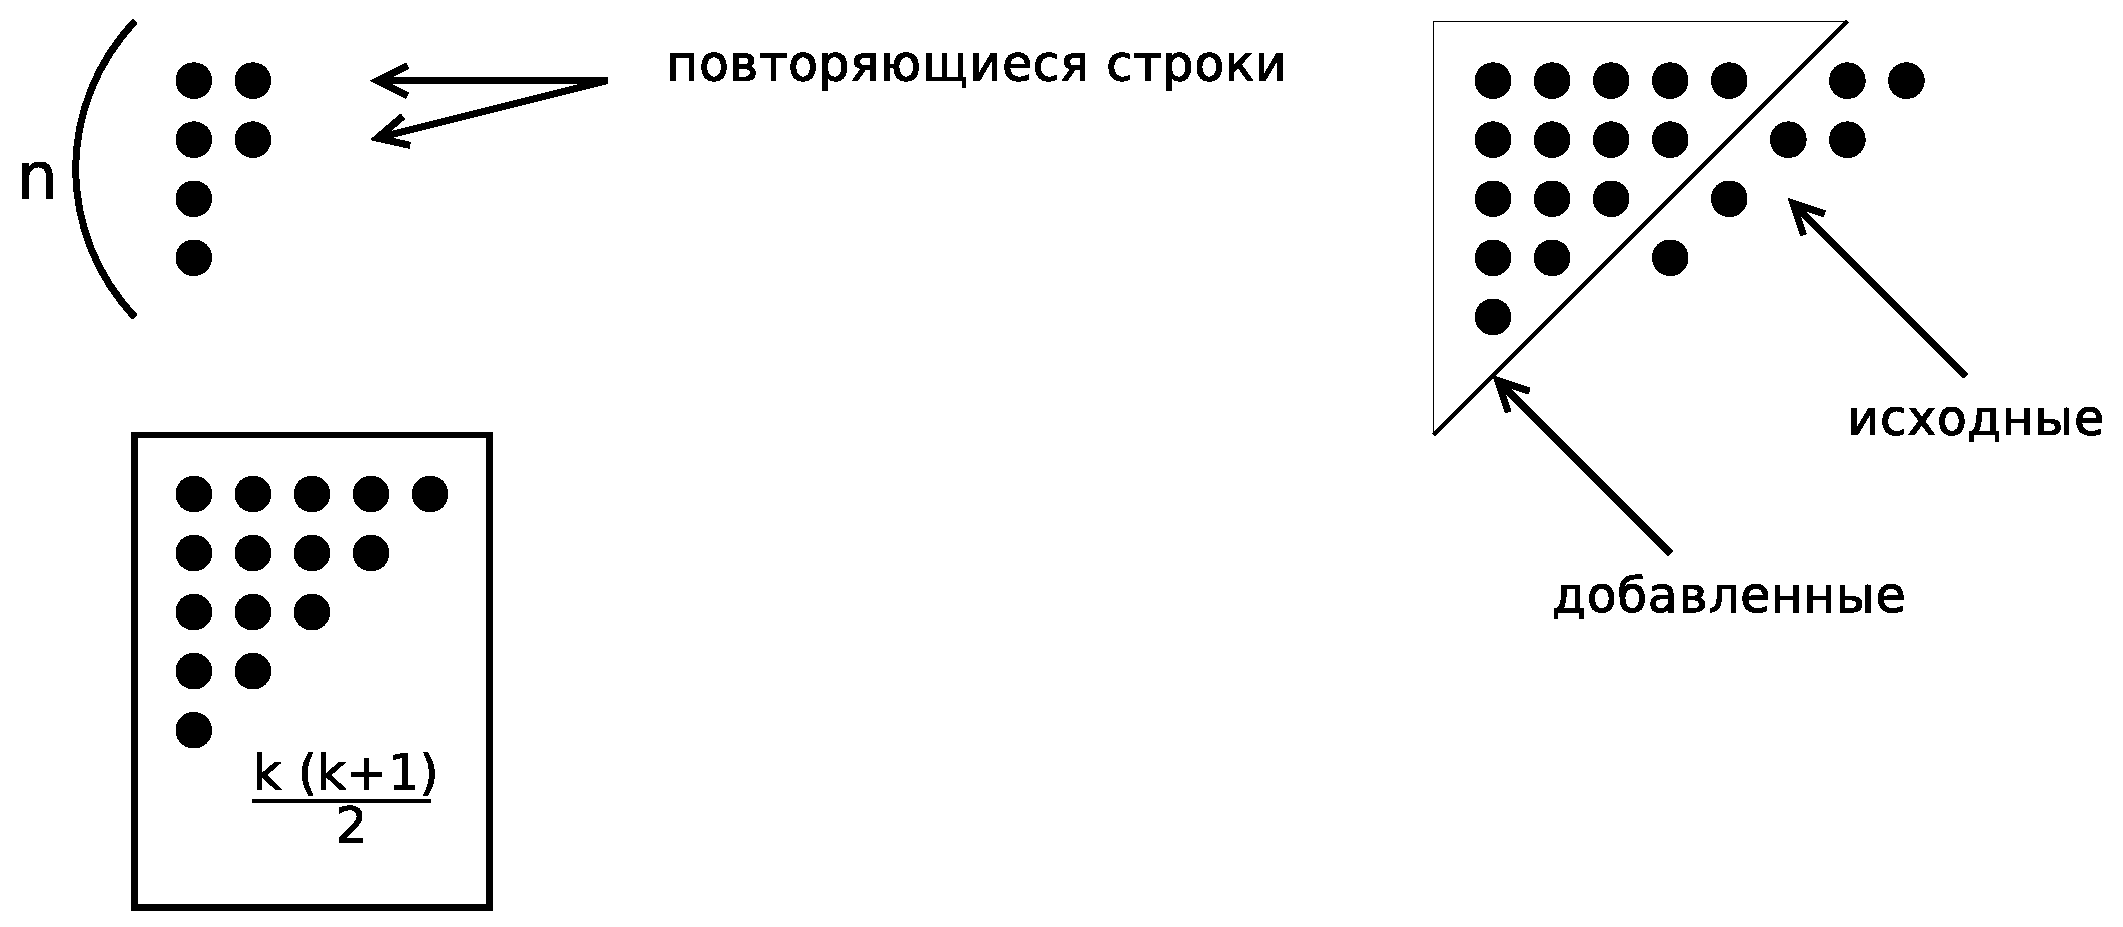
\includegraphics[width=0.8\linewidth]{ferre1}}
\caption{Преобразование диаграммы Ферре}
\label{img::ferre1}
\end{figure}

Таким образом добавив треугольник из $\frac{k \left(k+1\right)}{2}$ точек избавляемся от повторов строк, а кроме того приводим число строк ровно к $k$.
Обратное преобразование тоже возможно (и в общем вполне очевидно), т. е. на самом деле мы установили биекцию и доказали требуемое утверждение.

Другое, уже гораздо более содержательное задание, построить производящую функцию для количества различных симметриченых относительно диагонали (ну по другому это не будет диаграммой Ферре) диаграмм.

В решении этой задачи главное способ обхода точек диаграммы, подходящий способ обхода приведен на рис. \ref{img::ferre2}

\begin{figure}[h]
\center{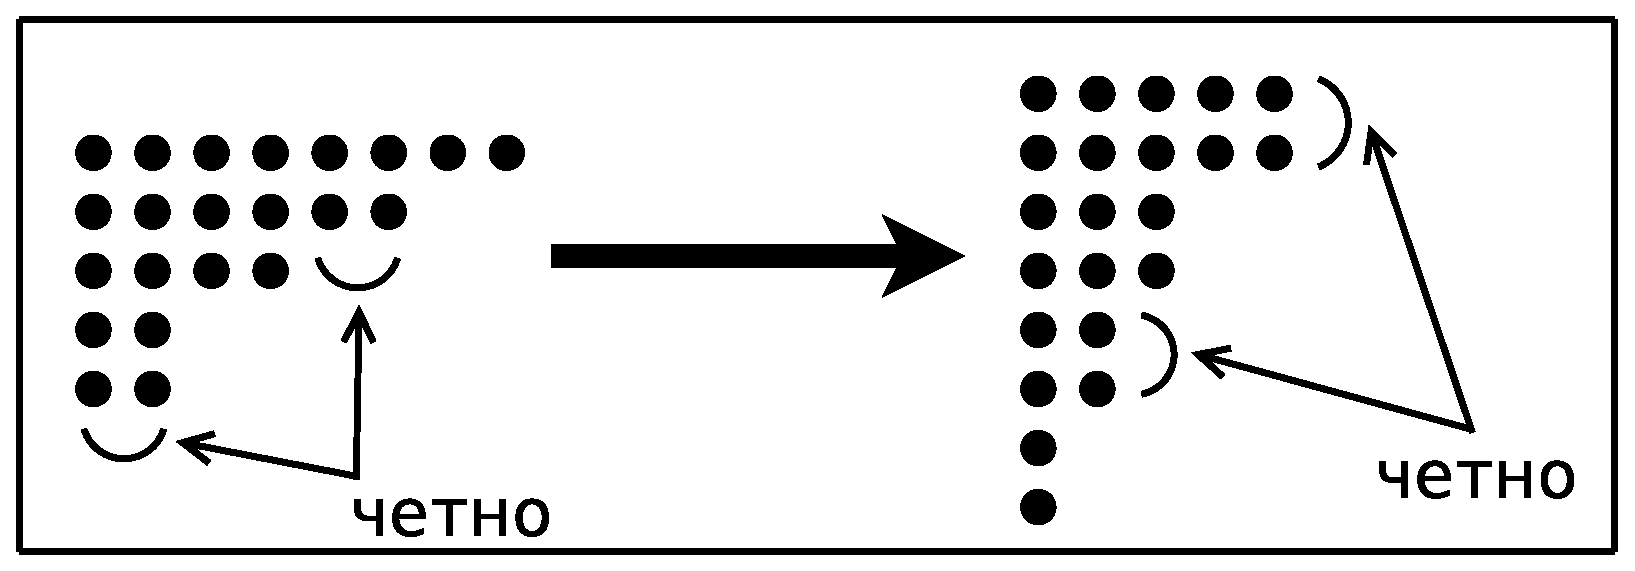
\includegraphics[width=0.8\linewidth]{ferre2}}
\caption{Обход диаграммы Ферре}
\label{img::ferre2}
\end{figure}

Итого свели исходную задачу к задаче о разбиении числа на различные нечетные слогаемые, а производящая функция для числа таких разбиений пишется сходу:
\[
	f\left(x\right) = \left(1+x\right)\left(1+x^3\right)...\left(1+x^{2k+1}\right)...
\]

Далее должна идти пентагональная теорема Эйлера, и если когда-то вдруг мне нечем будет заняться, и я из благороднейших побуждений и по доброте душевной не поленюсь и нарисую картинки диаграмм Ферре для частных случаев доказательства пентагональной теоремы, то оно конечно же здесь появится... Но вероятность этого мала) Всем спасибо, увидимся на следующей неделе.
